\section{Exercise one}

In this problem, we'll analyze the execution of a code segment on a single-issue out-of-order processor.
\begin{figure}[H]
    \centering
    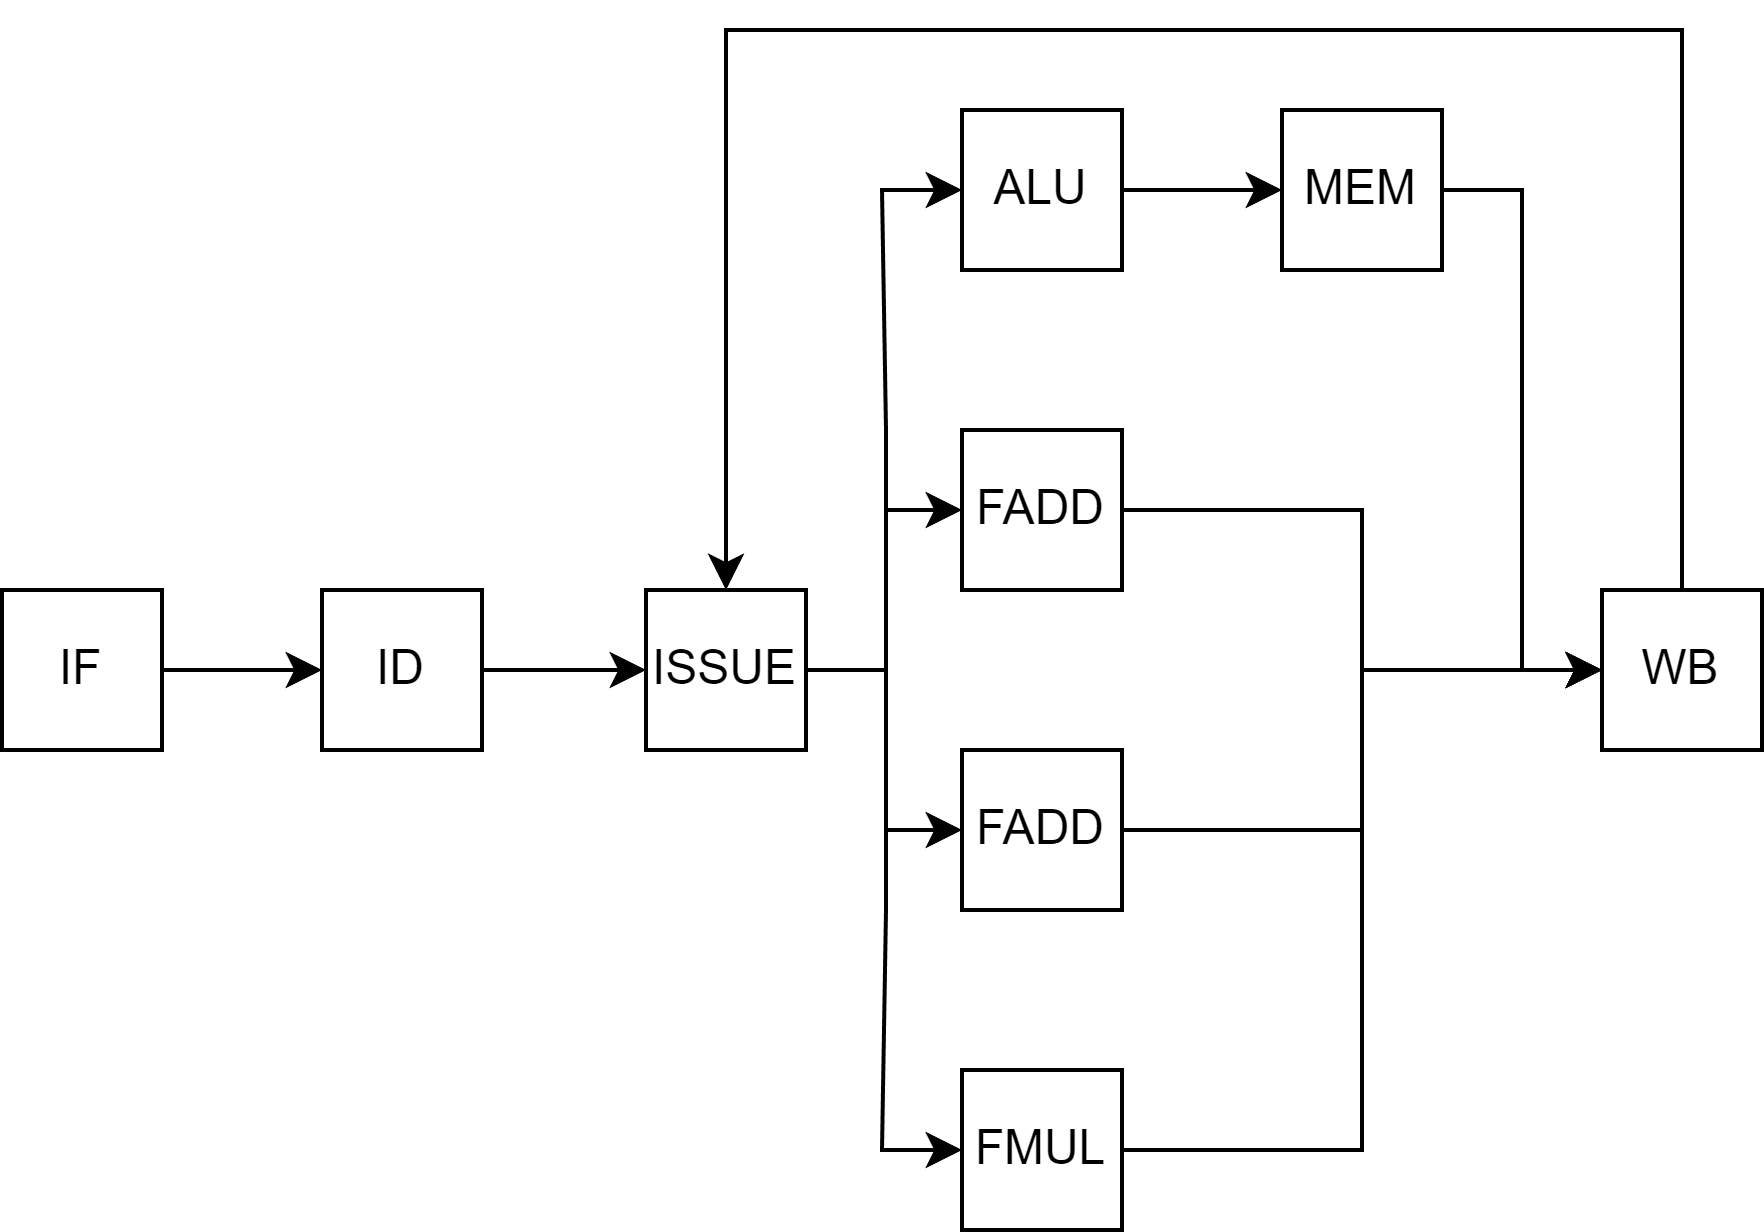
\includegraphics[width=0.75\linewidth]{images/complex.png}
\end{figure} 
Consider now the code:
\begin{verbatim}
I1 lw.d $F3,B($R0)
I2 add.d $F2,$F2,$F3
I3 mul.d $F5,$F4,$F4
I4 addi $R0,$R0,8
I5 lw.d $F3,B($R0)
I6 add.d $F2,$F3,$F5
\end{verbatim}
Examine each conflict taking into account the following operation durations:
\begin{itemize}
    \item Arithmetic logic unit operations: one cycle.
    \item Memory operations: three cycles.
    \item Floating point addition: three cycles.
    \item Floating point multiplication: five cycles.
\end{itemize}

\subsection*{Solution}
The conflicts are: 
\begin{itemize}
    \item RAW dependencies between instructions one and two, involving register \$F3.
    \item WAR conflict between instruction one and instructions one and four, concerning register \$R0.
    \item WAW conflict between instruction one and instructions one and five, affecting register \$F3.
    \item WAR conflict between instruction two and instructions two and five, regarding register \$F3.
    \item RAW dependency between instructions four and five, involving register \$R0.
    \item RAW dependency between instructions three and six, involving register \$F5.
    \item WAW conflict between instruction two and instructions two and six, impacting register \$F2.
    \item RAW dependency between instructions five and six, involving register \$F3.
\end{itemize}

A possible execution is: 
\begin{table}[H]
    \resizebox{\textwidth}{!}{%
    \begin{tabular}{c|cccccccccccccccccccc}
    \textbf{Instruction} & \textbf{C1} & \textbf{C2} & \textbf{C3} & \textbf{C4} & \textbf{C5} & \textbf{C6} & \textbf{C7} & \textbf{C8} & \textbf{C9} & \textbf{C10} & \textbf{C11} & \textbf{C12} & \textbf{C13} & \textbf{C14} & \textbf{C15} & \textbf{C16} & \textbf{C17} & \textbf{C18} & \textbf{C19} & \textbf{C20} \\ \hline
    \textit{1}           & F           & D           & IS          & E1          & E2          & E3          & W           &             &             &              &              &              &              &              &              &              &              &              &              &              \\
    \textit{2}           &             & F           & D           & \underline{S}     & \underline{S}     & \underline{S}     & IS          & E1          & E2          & E3           & W            &              &              &              &              &              &              &              &              &              \\
    \textit{3}           &             &             & F           & \underline{S}     & \underline{S}     & \underline{S}     & D           & IS          & E1          & E2           & E3           & E4           & E5           & W            &              &              &              &              &              &              \\
    \textit{4}           &             &             &             & \underline{S}     & \underline{S}     & \underline{S}     & F           & D           & IS          & E            & \underline{S}      & W            &              &              &              &              &              &              &              &              \\
    \textit{5}           &             &             &             &             &             &             &             & F           & \underline{S}     & D            & \underline{S}      & IS           & E1           & E2           & E3           & W            &              &              &              &              \\
    \textit{6}           &             &             &             &             &             &             &             &             & \underline{S}     & F            & \underline{S}      & D            & \underline{S}      & \underline{S}      & \underline{S}      & IS           & E1           & E2           & E3           & W           
    \end{tabular}%
    }
\end{table}
If we assume that the issue stage is a buffer with an unlimited capacity to hold instructions awaiting execution:
\begin{table}[H]
    \resizebox{\textwidth}{!}{%
    \begin{tabular}{c|cccccccccccccccccccc}
    \textbf{Instruction} & \textbf{C1} & \textbf{C2} & \textbf{C3} & \textbf{C4} & \textbf{C5} & \textbf{C6} & \textbf{C7} & \textbf{C8} & \textbf{C9} & \textbf{C10} & \textbf{C11} & \textbf{C12} & \textbf{C13} & \textbf{C14} & \textbf{C15} & \textbf{C16} & \textbf{C17} & \textbf{C18} & \textbf{C19} & \textbf{C20} \\ \hline
    \textit{1}           & F           & D           & IS          & E1          & E2          & E3          & W           &             &             &              &              &              &              &              &              &              &              &              &              &              \\
    \textit{2}           &             & F           & D           & \underline{S}     & \underline{S}     & \underline{S}     & IS          & E1          & E2          & E3           & W            &              &              &              &              &              &              &              &              &              \\
    \textit{3}           &             &             & F           & D           & \underline{S}     & \underline{S}     & \underline{S}     & IS          & E1          & E2           & E3           & E4           & E5           & W            &              &              &              &              &              &              \\
    \textit{4}           &             &             &             & D           & \underline{S}     & D           & \underline{S}     & \underline{S}     & IS          & E            & \underline{S}      & W            &              &              &              &              &              &              &              &              \\
    \textit{5}           &             &             &             &             & \underline{S}     & F           & \underline{S}     & \underline{S}     & \underline{S}     & D            & \underline{S}      & IS           & E1           & E2           & E3           & W            &              &              &              &              \\
    \textit{6}           &             &             &             &             &             &             & \underline{S}     & \underline{S}     & \underline{S}     & F            & D      & \underline{S}      & \underline{S}      & \underline{S}      & \underline{S}      & IS           & E1           & E2           & E3           & W           
    \end{tabular}%
    }
\end{table}